\documentclass{standalone}
\usepackage{graphicx}	
\usepackage{amssymb, amsmath, amsthm}
\usepackage{color}

\usepackage{tikz}
\usetikzlibrary{arrows.meta}

\definecolor{light}{RGB}{220, 188, 188}
\definecolor{mid}{RGB}{185, 124, 124}
\definecolor{dark}{RGB}{143, 39, 39}
\definecolor{highlight}{RGB}{180, 31, 180}
\definecolor{gray10}{gray}{0.1}
\definecolor{gray20}{gray}{0.2}
\definecolor{gray30}{gray}{0.3}
\definecolor{gray40}{gray}{0.4}
\definecolor{gray60}{gray}{0.6}
\definecolor{gray70}{gray}{0.7}
\definecolor{gray80}{gray}{0.8}
\definecolor{gray90}{gray}{0.9}
\definecolor{gray95}{gray}{0.95}

% #1: x
% #2: y
% #3: fillcolor
% #4: text
\newcommand{\textbox}[4]{
  \fill[rounded corners=4pt, fill=#3, text=white] 
    (#1 - \Dx, #2 - \Dy) rectangle (#1 + \Dx, #2 + \Dy)
  node[midway, yshift=0, align=center] { #4 };
}

% #1: x1
% #2: y1
% #3: x2
% #4: y2
\newcommand{\prettyarrow}[4]{
  \draw[color=black, -{Stealth[length=10pt, width=14pt]}, 
        line width=5, shorten >=-1pt] 
    (#1, #2) -- (#3, #4);
  \draw[color=white, -{Stealth[length=5pt, width=7pt]}, 
        line width=2, shorten >=1.25pt]
    (#1, #2) -- (#3, #4);
}

\begin{document}

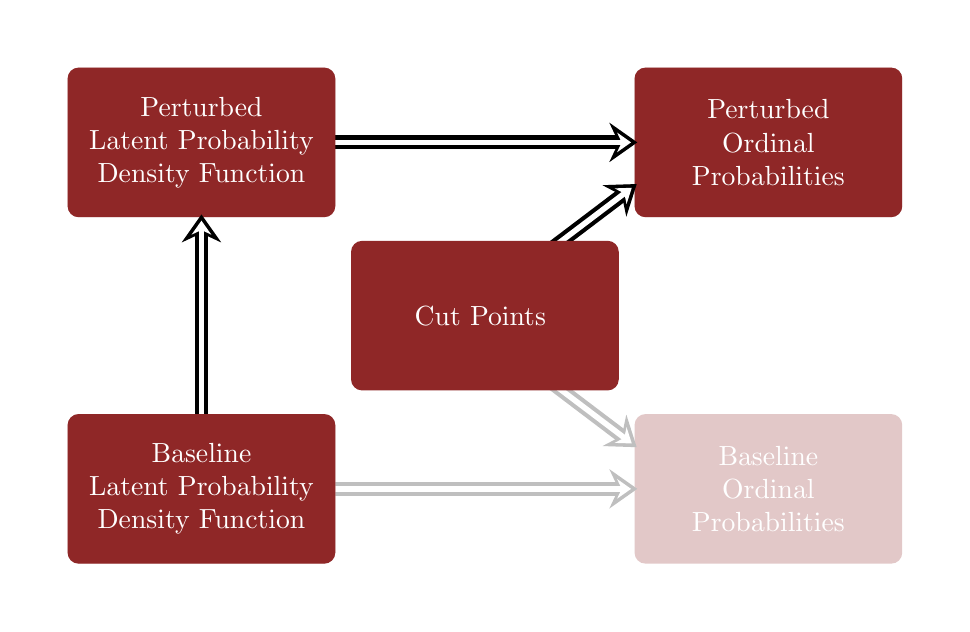
\begin{tikzpicture}
  % Size
  \pgfmathsetmacro{\Dx}{1.7}
  \pgfmathsetmacro{\Dy}{0.95}
  
  % Positioning
  \pgfmathsetmacro{\dx}{1.8}
  \pgfmathsetmacro{\dy}{1.1}
  \pgfmathsetmacro{\epsilon}{0.5}
  
  \draw[white]           (-2 * \dx - \Dx - \epsilon, -2 * \dy - \Dy - \epsilon) 
               rectangle (+2 * \dx + \Dx + \epsilon, +2 * \dy + \Dy + \epsilon);


  \textbox{+2 * \dx}{+2 * \dy}{dark}{Perturbed\\Ordinal\\Probabilities}
  
  \prettyarrow{0.5 * \Dx}{0.9 * \Dy}{2 * \dx - \Dx}{+1.5 * \dy}
  \prettyarrow{-2 * \dx + \Dx}{+2 * \dy}{2 * \dx - \Dx}{+2 * \dy}

  \textbox{-2 * \dx}{+2 * \dy}{dark}{Perturbed\\Latent Probability\\Density Function}
  
  \textbox{+2 * \dx}{-2 * \dy}{dark}{Baseline\\Ordinal\\Probabilities}  
    
  \prettyarrow{0.5 * \Dx}{-0.9 * \Dy}{2 * \dx - \Dx}{-1.5 * \dy}
  \prettyarrow{-2 * \dx + \Dx}{-2 * \dy}{2 * \dx - \Dx}{-2 * \dy}
  
  \prettyarrow{-2 * \dx}{-2 * \dy + \Dy}{-2 * \dx}{+2 * \dy - \Dy}
  
  \textbox{-2 * \dx}{-2 * \dy}{dark}{Baseline\\Latent Probability\\Density Function}

  \fill[white, opacity=0.75]           
              (-2 * \dx - \Dx - \epsilon, -2 * \dy - \Dy - \epsilon) 
    rectangle (+2 * \dx + \Dx + \epsilon, +2 * \dy + \Dy + \epsilon);

  \textbox{+2 * \dx}{+2 * \dy}{dark}{Perturbed\\Ordinal\\Probabilities}
  
  \prettyarrow{0.5 * \Dx}{0.9 * \Dy}{2 * \dx - \Dx}{+1.5 * \dy}
  \prettyarrow{-2 * \dx + \Dx}{+2 * \dy}{2 * \dx - \Dx}{+2 * \dy}

  \textbox{-2 * \dx}{+2 * \dy}{dark}{Perturbed\\Latent Probability\\Density Function}
  
  %\textbox{+2 * \dx}{-2 * \dy}{dark}{Baseline\\Ordinal\\Probabilities}  
    
  %\prettyarrow{0.5 * \Dx}{-0.9 * \Dy}{2 * \dx - \Dx}{-1.5 * \dy}
  %\prettyarrow{-2 * \dx + \Dx}{-2 * \dy}{2 * \dx - \Dx}{-2 * \dy}
  
  \prettyarrow{-2 * \dx}{-2 * \dy + \Dy}{-2 * \dx}{+2 * \dy - \Dy}
  
  \textbox{-2 * \dx}{-2 * \dy}{dark}{Baseline\\Latent Probability\\Density Function}

  \textbox{0}{0}{dark}{Cut Points}

    
\end{tikzpicture}

\end{document}  